\section{Stage 4: IDE Extension} \label{sec:work_stage4_extension_build}

The last \st{stage was to build an} \wo{componente is the} extension for an IDE. \wo{In this project, we choose the} VSCode. \wo{Dê um bom motivo de ser o vscode aqui.} This extension allows the user to have a better understanding of how much energy the code is consuming, and what are the methods, and variables that most affect it.
When opening the extension side page, it contains sliders that can change the input values, and it has the estimate button, to predict the energy.
\st{The sliders are updated when the document is saved.}%, rather than on every change, to prevent performance slowdowns.

The extension analyzes the user's Java files, identifies all the methods used, and matches them against a set of pre-trained models. Then it finds which variables affect those methods, meaning the variables that are the inputs to the method. For example, in \texttt{list.add(i)}  the inputs and important variables are \texttt{list} and \texttt{i} \wo{pela frase anterior, tinha percebido que eram só os inputs. \texttt{list} não é um input.}.
The extension does this to every method it finds \wo{in the source code} and groups it by method. In the end it creates groups of input variables for each method, displaying it in sliders. The sliders allow the user to change the input values and when pressing the estimate button and, \st{depending on the changed values} \wo{based on the values}, it will change the energy estimation.

If a method calls another user-defined method that already has an assigned energy cost (\st{but is not a trained method} \wo{but was not used to train the machine learning models}), then the calling method will also include that energy cost. This part was done by first analyzing individual methods for the model-trained methods and get their base energy. In a second iteration, each method is traversed to determine which calls are made, how many calls are made, and whether the calls are inside or outside loops. With this information, the total energy cost of each method could be calculated, accounting for both direct and indirect calls to model-trained methods.

When a model-trained method or a user-defined method are called inside a loop, a new slider appears to represent the loop size. The method’s energy cost is multiplied by this loop size. In the case of nested loops, the energy cost is multiplied by the product of all nested loop sizes. Note that only methods and variables that affect the energy appear on the panel.

This extension can help understand how much energy the code is using.
For example, \st{this small code} the snippet in Listing~\ref{lst:Java_program_to_count_word_frequencies_in_a_string} \st{that} counts how many times each word appears in a given text string, can be estimated for how much energy it uses.

\begin{listing}[htbp]
\noindent\rule{\linewidth}{0.4pt}
\begin{minted}[linenos, fontsize=\small, frame=none, bgcolor=white,breaklines=true,breakanywhere=true]{Java}
    public class WordFrequency {
    public static HashMap<String, Integer> countWordFrequency(String text) {
        String[] words = text.toLowerCase().split("\\W+");
        HashMap<String, Integer> frequencyMap = new HashMap<>();
        for (String word : words) {
            if (word.isEmpty()) continue; 
            frequencyMap.put(word, frequencyMap.getOrDefault(word, 0) + 1);
        }
        return frequencyMap;
    }
    public static void main(String[] args) {
        String input = "Java is simple. Java is powerful.";
        HashMap<String, Integer> result = countWordFrequency(input);
        System.out.println(result);
    }
}
\end{minted}
\noindent\rule{\linewidth}{0.4pt}
\caption{Java program to count word frequencies in a string}            
\label{lst:Java_program_to_count_word_frequencies_in_a_string}
\end{listing}

\st{Using the energy prediction extension it is possible to understand how much energy this code uses, as it can be seen in the Figure}~\ref{fig:extension_example1}.
\wo{Figure~\ref{fig:extension_example1} illustrates how the extension displays the energy consumption of the code in Listing~\ref{lst:Java_program_to_count_word_frequencies_in_a_string}.} In the figure two methods \st{can be seen, and their energy is displayed} \wo{\texttt{countWordFrequency(String)} and \texttt{main(String[])} can be seen, next to their energy consumption estimations}. \st{also one of the containers has the important variables that might affect the energy of the code} \wo{Its also shown under the box with the method's name, the important variables that can affect energy consumption}. For instance, in the method \texttt{countWordFrequency(String)} it can be seen that the size of the variables \texttt{word} and \texttt{frequencyMap} can change the energy usage. Also, the loop size is taken into account, and the number operations performed will impact the energy significantly.

\wo{reescrever →}
The two variables shown in the Figure~\ref{fig:extension_example1}, show up because of the method \texttt{Map.put(Object,Object)}, which means it will have three inputs. The first one is the collection input, (i.e \texttt{frequencyMap}), the second one is the first Object which is the variable \texttt{word} and the last Object is not a variable, so it does not appear in the extension. \wo{← não percebi o que estás a tentar dizer aqui.}


\begin{figure}[htbp]
  \centering
  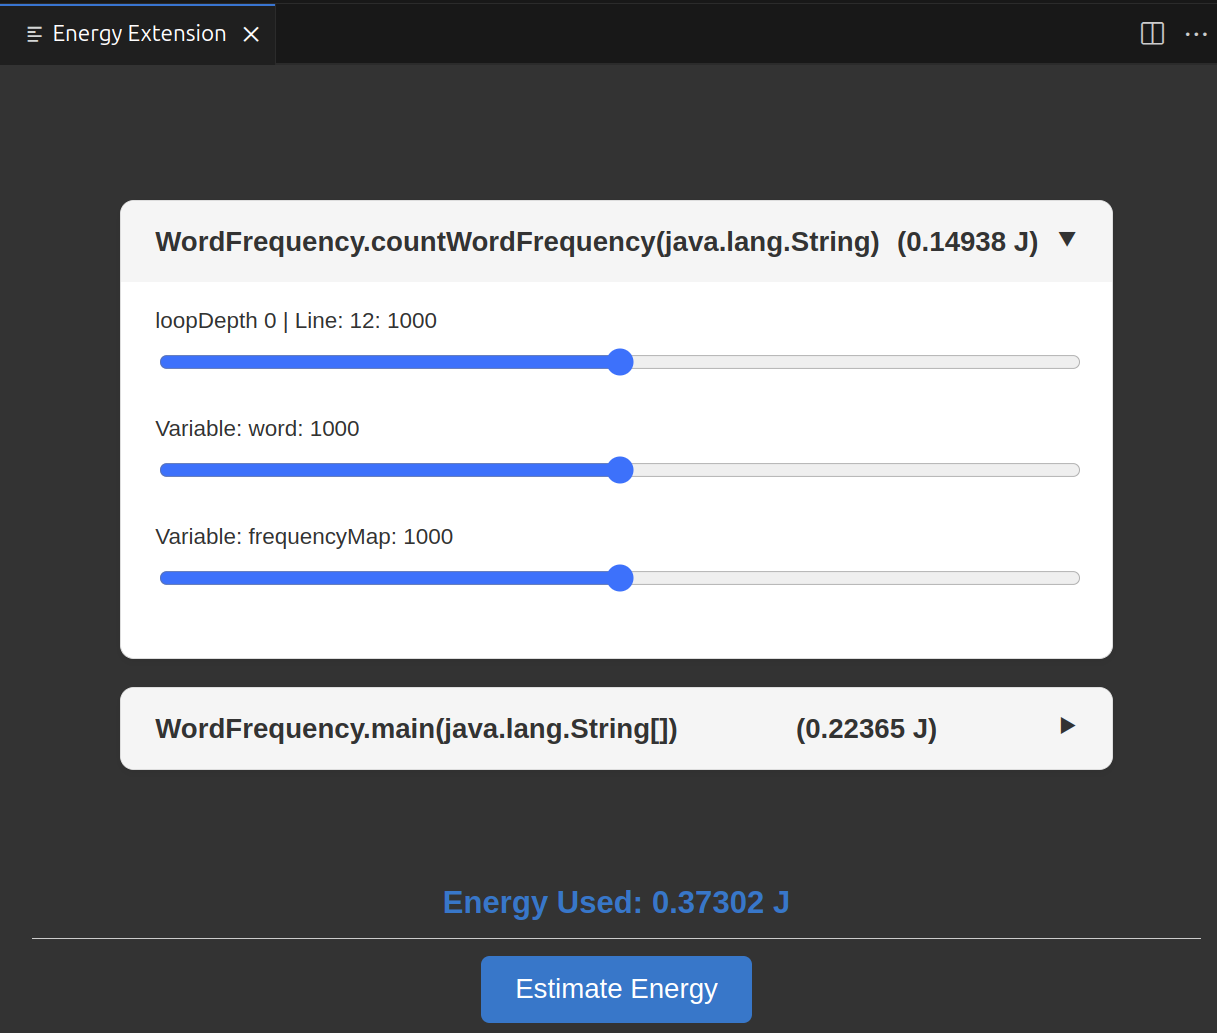
\includegraphics[width = .8 \textwidth]{figures/extension_example1.png}
  \caption{Extension example HashMap}
  \label{fig:extension_example1}
\end{figure}


\wo{Another example can be see in the Figure~\ref{fig:extension_example2}, where the same code is used, but instead of using a \texttt{HashMap} it uses a \texttt{TreeMap}. The energy consumption is different, as the model was trained to understand that the \texttt{TreeMap} consumes more energy than the \texttt{HashMap}.}

%If, for instance, instead of using \texttt{HashMap}, \texttt{TreeMap} is used, the energy differences can easily be noticed in the Figure~\ref{fig:extension_example2}. This shows a great example of how two implementations of the same collection can differ in energy. It can also be used to compare different method implementations, that achieve the same output but rely on different approaches.



\begin{figure}[htbp]
  \centering
  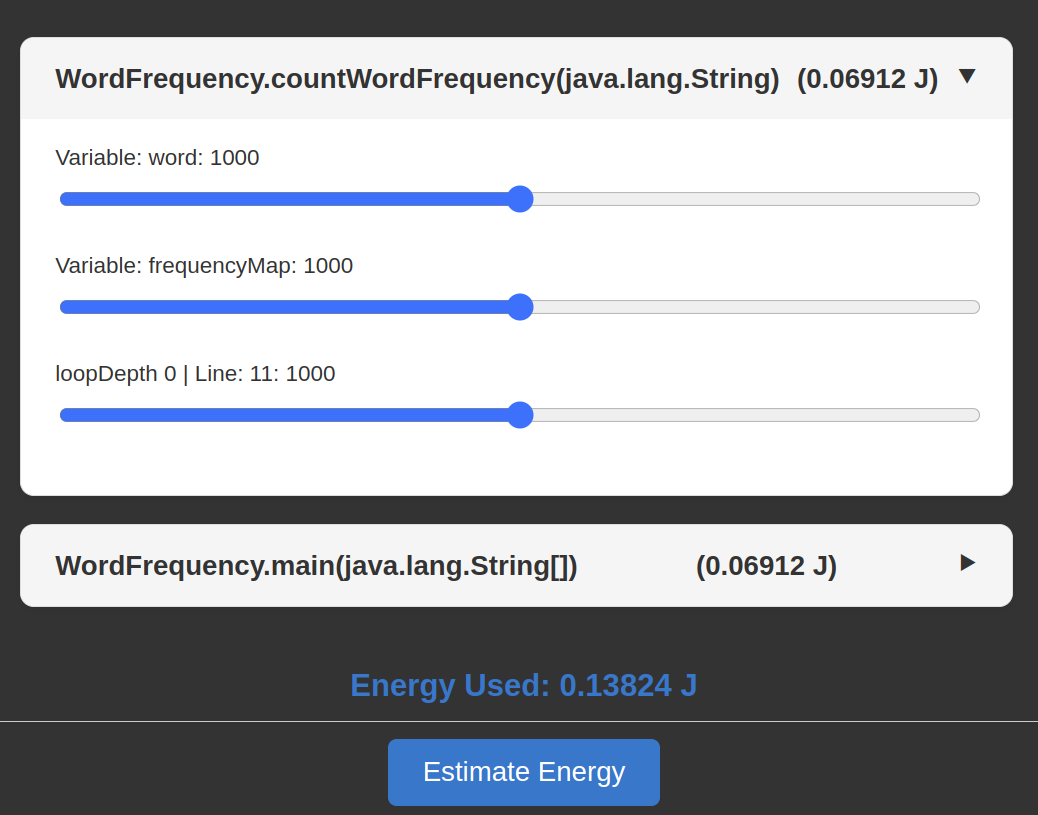
\includegraphics[width = .8 \textwidth]{figures/extension_example2.png}
  \caption{Extension example TreeMap}
  \label{fig:extension_example2}
\end{figure}

There is also a feature that can help the user understand how the energy changes. When the mouse hovers through some methods, it is possible to see the mathematical expression utilized for the calculations. The Figure~\ref{fig:extension_expression_example} shows how the expression is displayed in the extension UI. It has the numbers that the model think are the best to predict the energy, and it has the features/variables that it affects the prediction the most. In this case the two variables are the size of the map collection and if there are any \texttt{TreeMap} collection being used. This can help understand what are the variables that actually impact the energy of the code. 


\begin{figure}[htbp]
  \centering
  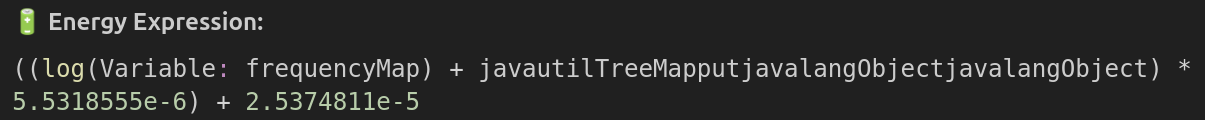
\includegraphics[width = .8 \textwidth]{figures/extension_expression_example.png}
  \caption{Expression for method Map.put(Object, Object)}
  \label{fig:extension_expression_example}
\end{figure}

{\color{blue}
Another useful feature is the line that spends more energy in each method. Being the line a user defined function or a model trained method, the line will appear highlighted, helping the developer in case of needing help on where to start when needing to refactor the code for energy efficiency. The example can be seen in the Figure~\ref{fig:most_expensive_line}.}

\begin{figure}[htbp]
  \centering
  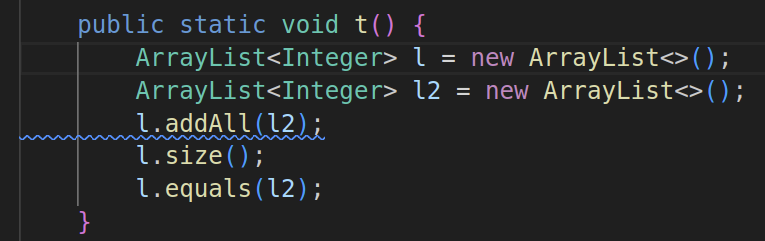
\includegraphics[width = .6 \textwidth]{figures/most_expensive_line.png}
  \caption{Most expensive line highlighted}
  \label{fig:most_expensive_line}
\end{figure}

The extension can be open in a Java project and gather the total energy used by the user made methods, allowing for a better understanding of the code energy impact. Naturally, the extension is limited by the set of pre-trained models it relies on. If a program uses methods that aren't covered by these models, the extension will report an energy usage of zero, which is inaccurate, as those methods still consume energy.

\wo{This highlights the importance of continuously expanding the set of pre-trained models to cover a wider range of methods and scenarios. As more energy profiles are collected, the models will be able to predict more accurately the energy consumption of the code.}

\wo{The extension is designed to be extensible, allowing for the addition of more energy profiles, features,  and models as they become available. This ensures that the entire frameowkr remains relevant and useful for developers as they work on increasingly complex projects.}